\chapter{Results}
\label{chapter:Results}

\begin{introduction}
    "The only source of knowledge is experience." - Albert Einstein
\end{introduction}

\section{Evolution of Software Development}

The software development process has undergone several important stages, each enhancing its functionality and usability. The figures below illustrate the application's progress, showcasing different phases of refinement as the project matured.

\subsection{Initial Stages: Basic Functionality and User Interaction}

The first figure (Figure \ref{fig:v1}) represents the early stages of development, where the primary focus was on creating a user-friendly interface for calculating average read depth and coverage metrics from a BAM file for a Single Gene. In this version, the application prominently features a two-step process where the user selects a BED file releated to de gene to analyse and one or more BAM files. These files are then processed to calculate key metrics, which are displayed in the results table below. This simple design allowed for efficient user interaction but was somewhat limited in terms of flexibility and scope.

At this stage, the core challenge was to ensure that the software could handle large genomic files while presenting the results in a clear and intuitive format. The layout emphasizes simplicity, making it easier for users to navigate through the two-step process. However, as the project progressed, the need for more advanced features became evident.

\begin{figure}[H]
    \centering
    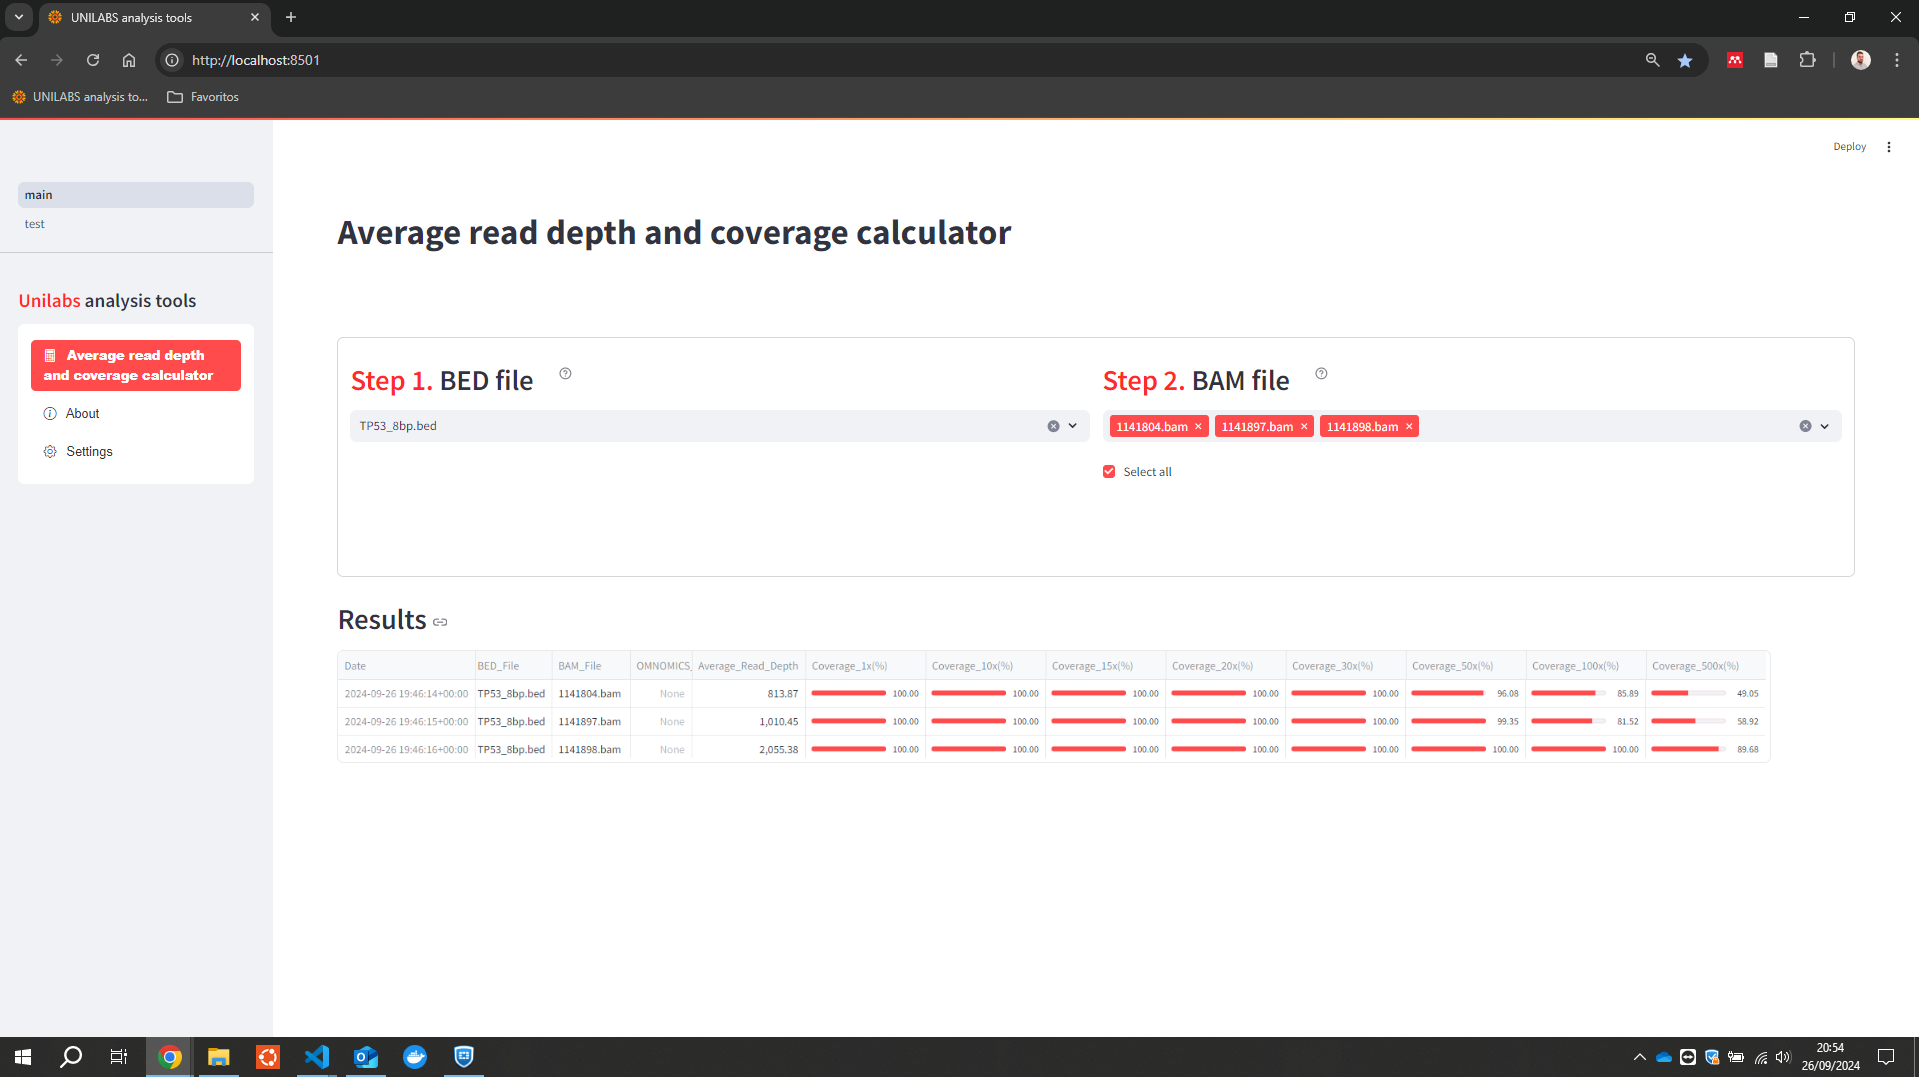
\includegraphics[width=1\textwidth]{figs/v1.png}
    \caption{First version of the GUI.} 
    \label{fig:v1}
\end{figure}

\subsection{Refinement: Introducing Flexibility and Multiple Analysis Modes}

In the second figure (Figure \ref{fig:v2}), the software has significantly evolved to include more detailed analysis options. The interface now presents multiple analysis types: \textit{Single Gene}, \textit{Gene Panel}, and \textit{Exome}, catering to different research needs. This flexibility represents a major shift from the earlier version, as it now allows users to select specific genome assemblies and regions of interest by using an universal BED file. Additionally, the results section has been split into tabs such as \textit{Overview} and \textit{Exon Details}, giving users the ability to drill down into the metrics for a single gene or explore exon-level coverage details. However, even though this last features were thinked to be used in this version, they only have been work fully in the last version of the software. 

\begin{figure}[H]
    \centering
    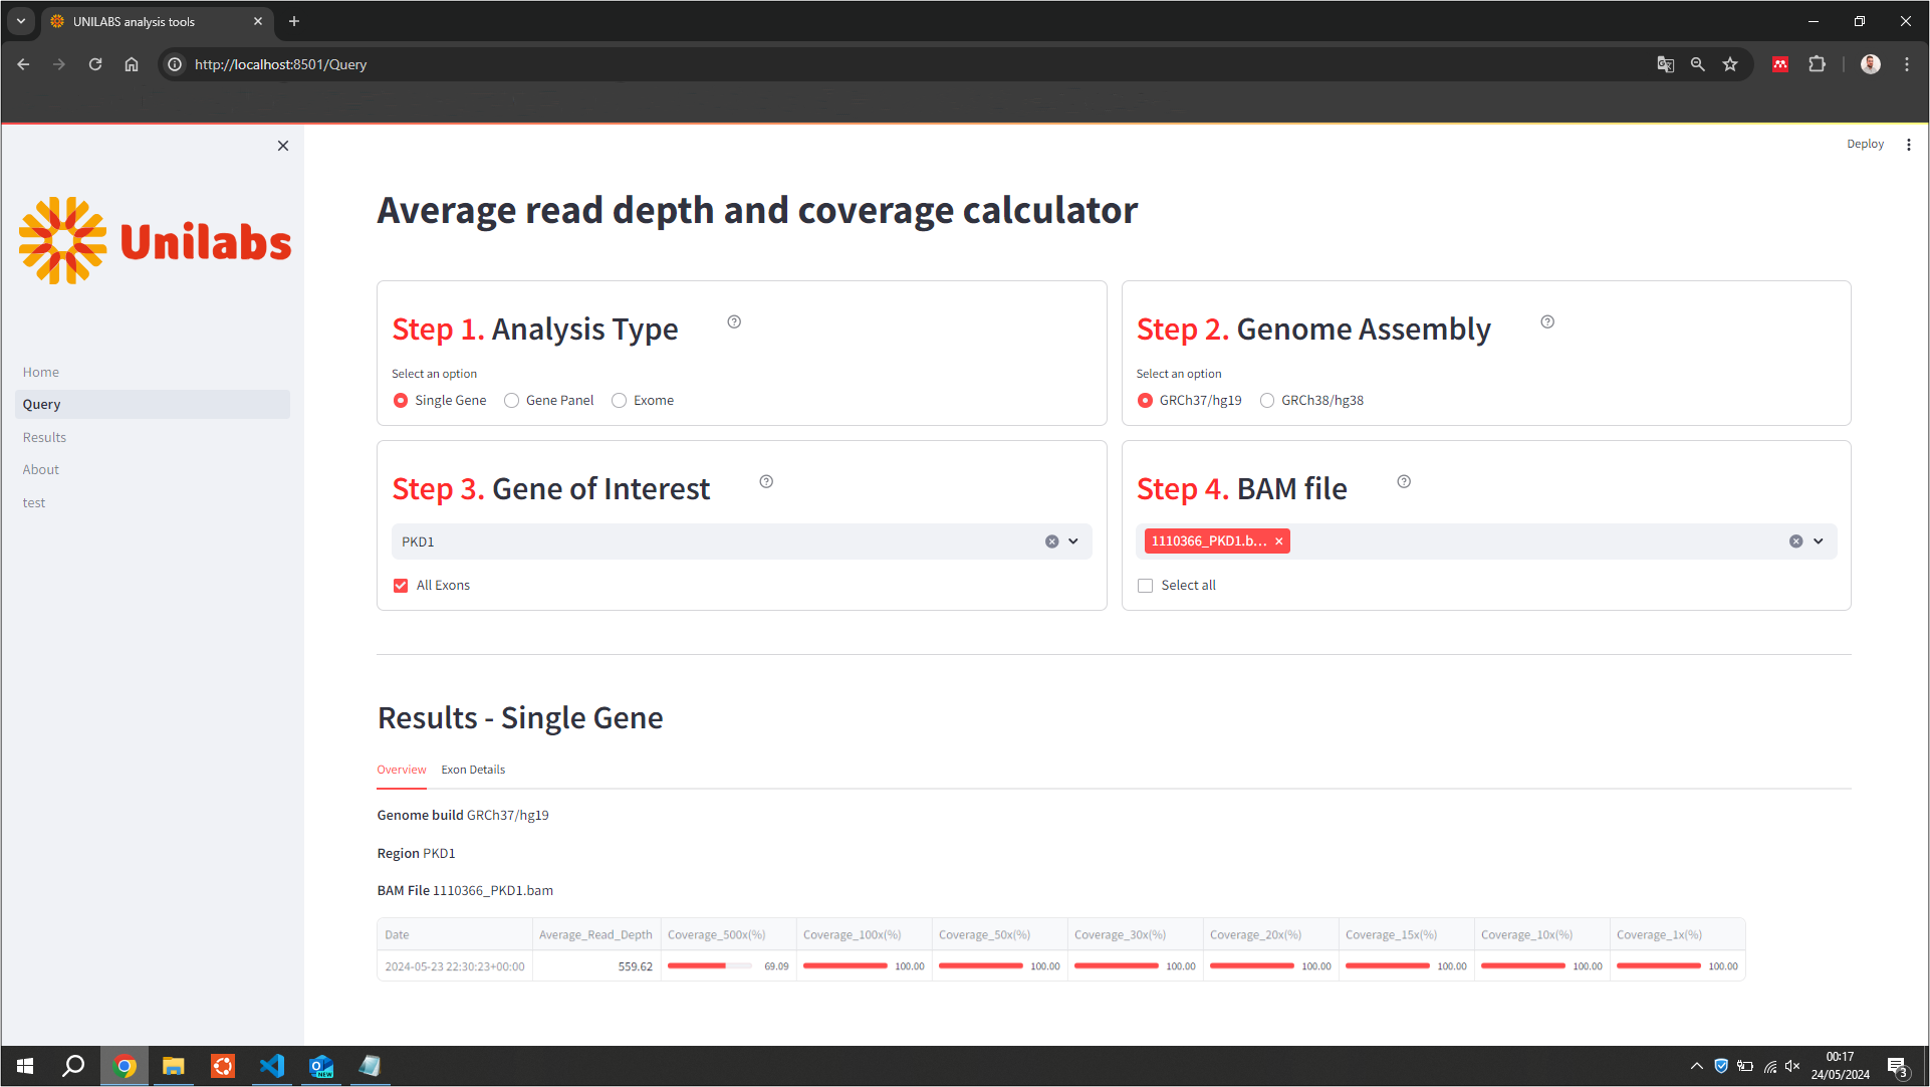
\includegraphics[width=1\textwidth]{figs/v2.png}
    \caption{Second version of the GUI.} 
    \label{fig:v2}
\end{figure}






\section{Real data test running}
\section{Test and validation}

De forma a validar a ferramenta, foram realizados testes com dados reais de sequenciação genómica. Os resultados obtidos foram comparados com os obtidos por outras ferramentas de análise de dados genómicos comerciais, como a \textit{Omnomics}. Foram reproduzidas as análises para Singles Gene e Gene Panel. 
No primeiro caso, para o mesmo ficheiro de alinhamento .bam, e usando como referência a mesma versaão do genoma humano (hg19), os resultados obtidos foram semelhantes como se pode observar na Figura

\section{Performance}


\section{Comparison with other tools}


\section{Users feedback}






